\begin{figure}[!ht]\centering
	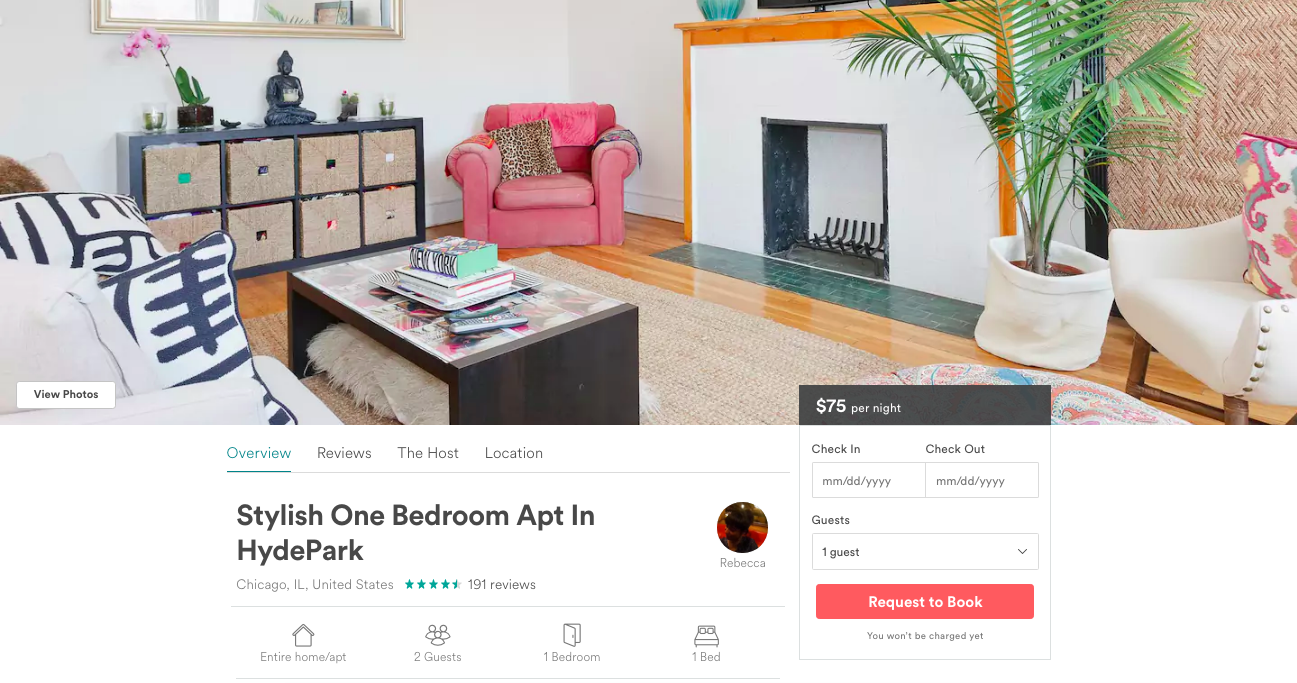
\includegraphics[width=.8\textwidth]{figures/sample1-cover}
	\caption{Sample listing page}
	\label{fig:listing}
\end{figure}

\begin{figure}[!ht]\centering
	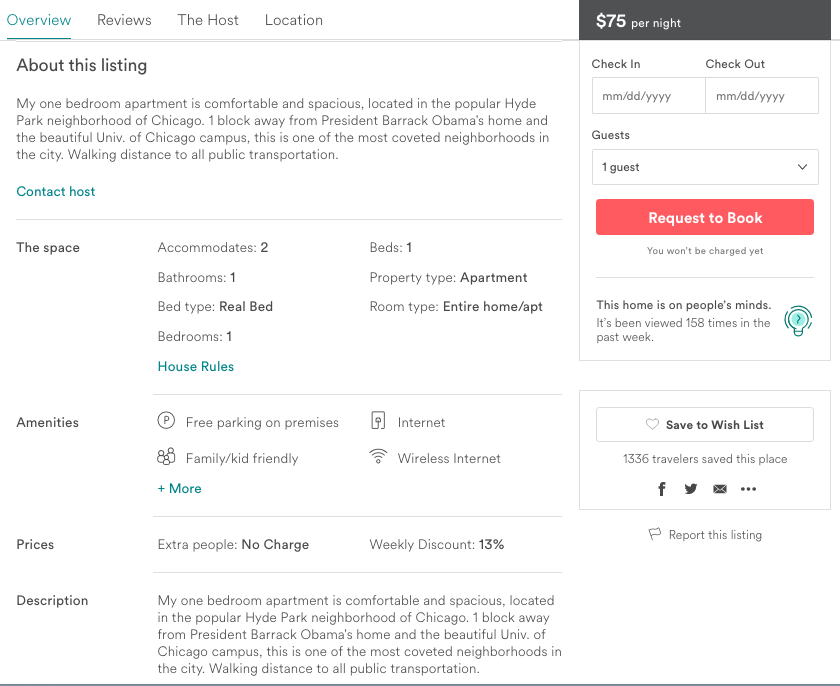
\includegraphics[width=.8\textwidth]{figures/sample2-property}
	\caption{Listing information}
	\label{fig:property}
\end{figure}

\begin{figure}[!ht]\centering
\includegraphics[width=.8\textwidth]{figures/sample3-reviews}
\caption{Review information}
	\label{fig:reviewinfo}
\end{figure}

\begin{figure}\centering
\includegraphics[width=.9\textwidth]{figures/sample4-host}
\caption{Host information}
	\label{fig:host}
\end{figure}

\begin{figure}\centering
\includegraphics[width=.8\textwidth]{figures/sample5-location}
\caption{Location information}
	\label{fig:location}
\end{figure}

\begin{figure}\centering
\includegraphics[width=.8\textwidth]{figures/chicago_city_neighborhoods}
\caption[City of Chicago neighborhoods]{City of Chicago neighborhoods, showing level of granularity of neighborhood controls}
	\label{fig:chicago}
\end{figure}


